
\newpage
\section{Numerical results}%
\label{sec:numerical_results}


\subsection{Numerical Results for CutCIP Biharmonic Equation  }%
\label{sub:numerical_results_for_cutcip_biharmonic_equation_}

\begin{itemize}
    \item EOC Test on circle and its configuration
        \begin{enumerate}[label=\arabic*)]
            \item Penalty parameters $\gamma , \gamma _{g1}, \gamma _{g2} = 20,10, 0.1$
            \item Background mesh $L = 3.11$ and circle $R=1$, flower $r0, r1 = L0.3, L0.1$
        \end{enumerate}
    \item Translation
        \begin{enumerate}[label=\arabic*)]
            \item Background mesh $L = 3.11$ and $R=1$
        \end{enumerate}
\end{itemize}


In this section will we provide a numerical study of the methods studied in Section \ref{sec:cutcip_biharmonic_problem}.

\subsubsection{EOC test}%
\label{ssub:eoc_test}

Here we consider the manufactured solution $l,r,m = (2, 1, 1) $ s.t.
\[
u_{\text{ex}}(x,y) = (x^2- y^2 -1) \sin\left(\frac{2\pi m}{l}x_1\right)\cos\left(\frac{2\pi r}{l}y\right)
\]
On a square background mesh $L=3.11$ with a circle domain of radius $R=1$.

\begin{table}
\begin{table}
  \begin{tabular}{rrrrrrrrr}
    \noalign{\hrule height 2pt}
    \textbf{$n$} & \textbf{$\Vert e \Vert_{L^2}$} & \textbf{EOC} & \textbf{$ \Vert e \Vert_{H^1}$} & \textbf{EOC} & \textbf{$\Vert e \Vert_{ a_h,* }$} & \textbf{EOC} & \textbf{Cond number} & \textbf{ndofs} \\\noalign{\hrule height 2pt}
    8 & 1.4E-01 & NaN & 7.3E-01 & NaN & 7.4E+00 & NaN & 1.7E+05 & 1.8E+02 \\
    16 & 3.4E-02 & 2.03 & 2.0E-01 & 1.87 & 3.8E+00 & 0.97 & 9.2E+05 & 4.8E+02 \\
    32 & 1.0E-02 & 1.74 & 4.9E-02 & 2.02 & 1.8E+00 & 1.06 & 6.6E+06 & 1.6E+03 \\
    64 & 2.7E-03 & 1.88 & 1.2E-02 & 2.03 & 9.0E-01 & 1.03 & 5.0E+07 & 5.6E+03 \\
    128 & 7.0E-04 & 1.97 & 3.1E-03 & 1.99 & 4.4E-01 & 1.01 & 3.9E+08 & 2.1E+04 \\
    256 & 2.2E-04 & 1.64 & 8.2E-04 & 1.90 & 2.2E-01 & 1.01 & 3.0E+09 & 8.1E+04 \\\noalign{\hrule height 2pt}
  \end{tabular}
\end{table}

\caption{Convergence rates for the Hessian-based method applied to the circular domain with side length $L=3.11$, using parameters $\gamma=20$, $\gamma_1=10$, and $\gamma_2=0.1$}
\end{table}

\begin{table}
\begin{table}
  \begin{tabular}{rrrrrrrrr}
    \noalign{\hrule height 2pt}
    \textbf{$n$} & \textbf{$\Vert e \Vert_{L^2}$} & \textbf{EOC} & \textbf{$ \Vert e \Vert_{H^1}$} & \textbf{EOC} & \textbf{$\Vert e \Vert_{ a_h,* }$} & \textbf{EOC} & \textbf{Cond number} & \textbf{ndofs} \\\noalign{\hrule height 2pt}
    8 & 1.4E-01 & NaN & 7.3E-01 & NaN & 7.4E+00 & NaN & 1.7E+05 & 1.8E+02 \\
    16 & 3.4E-02 & 2.03 & 2.0E-01 & 1.87 & 3.8E+00 & 0.97 & 9.2E+05 & 4.8E+02 \\
    32 & 1.0E-02 & 1.74 & 4.9E-02 & 2.02 & 1.8E+00 & 1.06 & 6.6E+06 & 1.6E+03 \\
    64 & 2.7E-03 & 1.88 & 1.2E-02 & 2.03 & 9.0E-01 & 1.03 & 5.0E+07 & 5.6E+03 \\
    128 & 7.0E-04 & 1.97 & 3.1E-03 & 1.99 & 4.4E-01 & 1.01 & 3.9E+08 & 2.1E+04 \\
    256 & 2.2E-04 & 1.64 & 8.2E-04 & 1.90 & 2.2E-01 & 1.01 & 3.0E+09 & 8.1E+04 \\\noalign{\hrule height 2pt}
  \end{tabular}
\end{table}

\caption{Convergence rates for the Laplacian-based method applied to the circular domain with side length $L=3.11$, using parameters $\gamma=20$, $\gamma_1=10$, and $\gamma_2=0.1$}
\end{table}
\begin{figure}\centering
\subfloat[]{\label{a}
        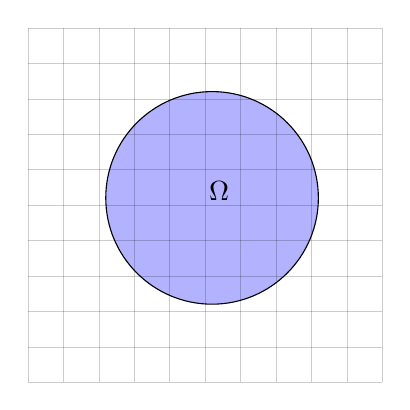
\begin{tikzpicture}[scale=0.9]

            % Domain is blue
            \fill[blue!30] (0.1, 0.1) circle (1.5cm);
            \draw[black] (0.1, 0.1) circle (1.5cm);
            \node at (0.2, 0.2) {$\Omega$};

            % Background mesh
            \foreach \i in {-2.5, -2, ..., 2.5} {
                \draw[line width=0.1pt, shift={(-2.5,\i)}, opacity=0.2] (0,0) -- (5,0);
                \draw[line width=0.1pt, shift={(\i,-2.5)},opacity=0.2] (0,0) -- (0,5);
            }

        \end{tikzpicture}

}\hfill
\subfloat[]{\label{b}
        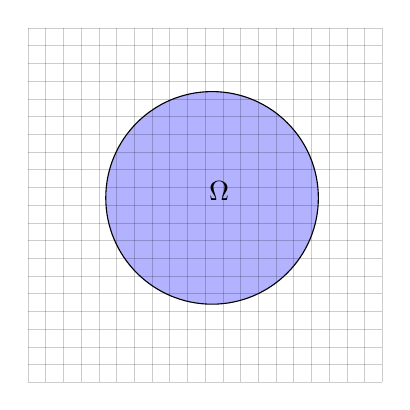
\begin{tikzpicture}[scale=0.9]

            % Domain is blue
            \fill[blue!30] (0.1, 0.1) circle (1.5cm);
            \draw[black] (0.1, 0.1) circle (1.5cm);
            \node at (0.2, 0.2) {$\Omega$};

            % Background mesh
            \foreach \i in {-2.5, -2.25, ..., 2.5} {
                \draw[line width=0.1pt, shift={(-2.5,\i)}, opacity=0.2] (0,0) -- (5,0);
                \draw[line width=0.1pt, shift={(\i,-2.5)},opacity=0.2] (0,0) -- (0,5);
            }

        \end{tikzpicture}


}
\hfill
\subfloat[]{\label{c}
        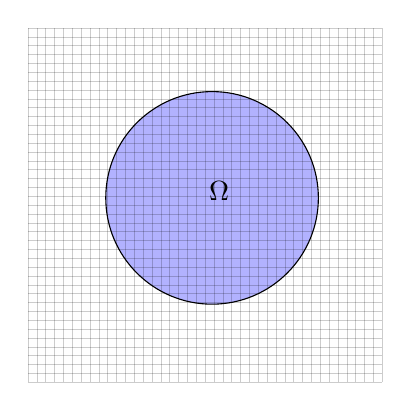
\begin{tikzpicture}[scale=0.9]

            % Domain is blue
            \fill[blue!30] (0.1, 0.1) circle (1.5cm);
            \draw[black] (0.1, 0.1) circle (1.5cm);
            \node at (0.2, 0.2) {$\Omega$};

            % Background mesh
            \foreach \i in {-2.5, -2.375, ..., 2.5} {
                \draw[line width=0.1pt, shift={(-2.5,\i)}, opacity=0.2] (0,0) -- (5,0);
                \draw[line width=0.1pt, shift={(\i,-2.5)},opacity=0.2] (0,0) -- (0,5);
            }

        \end{tikzpicture}
}
    \caption{Illustration of the domain $\Omega $ defined as a circle with radius $R$. The background mesh is a square domain with side lengths $L$ with three refinements of the mesh size $h$.}
\end{figure}


Here we consider the manufactured solution $l,r,m = (2, 1, 1) $ s.t.
\[
u_{\text{ex}}(x,y) = \sin\left(\frac{2\pi m}{l}x_1\right)\cos\left(\frac{2\pi r}{l}y\right)
\]
on the flower domain for the Laplace equation.

\begin{table}
\begin{table}
  \begin{tabular}{rrrrrrrrr}
    \noalign{\hrule height 2pt}
    \textbf{$n$} & \textbf{$\Vert e \Vert_{L^2}$} & \textbf{EOC} & \textbf{$ \Vert e \Vert_{H^1}$} & \textbf{EOC} & \textbf{$\Vert e \Vert_{ a_h,* }$} & \textbf{EOC} & \textbf{Cond number} & \textbf{ndofs} \\\noalign{\hrule height 2pt}
    8 & 1.4E-01 & NaN & 7.3E-01 & NaN & 7.4E+00 & NaN & 1.7E+05 & 1.8E+02 \\
    16 & 3.4E-02 & 2.03 & 2.0E-01 & 1.87 & 3.8E+00 & 0.97 & 9.2E+05 & 4.8E+02 \\
    32 & 1.0E-02 & 1.74 & 4.9E-02 & 2.02 & 1.8E+00 & 1.06 & 6.6E+06 & 1.6E+03 \\
    64 & 2.7E-03 & 1.88 & 1.2E-02 & 2.03 & 9.0E-01 & 1.03 & 5.0E+07 & 5.6E+03 \\
    128 & 7.0E-04 & 1.97 & 3.1E-03 & 1.99 & 4.4E-01 & 1.01 & 3.9E+08 & 2.1E+04 \\
    256 & 2.2E-04 & 1.64 & 8.2E-04 & 1.90 & 2.2E-01 & 1.01 & 3.0E+09 & 8.1E+04 \\\noalign{\hrule height 2pt}
  \end{tabular}
\end{table}

\caption{
Convergence rates for the Laplace-based method applied to the flower-shaped domain with side length $L=3.11$, using parameters $\gamma=20$, $\gamma_1=10$, and $\gamma_2=0.1$.
}
\end{table}




